\documentclass[review]{elsarticle}

\usepackage{lineno,hyperref}
\modulolinenumbers[5]

% for alg.
\usepackage{algorithm}
\usepackage{algpseudocode}
\usepackage{enumitem}
\usepackage{balance}
\usepackage{subfig}
\usepackage{color}
\def\algbackskip{\hskip\dimexpr-\algorithmicindent+\labelsep}
\def\LState{\State \algbackskip}

% for table.
\usepackage{multirow, array, amsmath}

% for Chinese
\usepackage{CJKutf8}

% cancel line
\usepackage{ulem}

\journal{Journal of \LaTeX\ Templates}

\newcommand{\replace}[1]{$\langle$\textit{#1}$\rangle$}
\newcommand{\HL}[1]{\textcolor[rgb]{1.00,0.00,0.00}{#1}}

%%%%%%%%%%%%%%%%%%%%%%%
%% Elsevier bibliography styles
%%%%%%%%%%%%%%%%%%%%%%%
%% To change the style, put a % in front of the second line of the current style and
%% remove the % from the second line of the style you would like to use.
%%%%%%%%%%%%%%%%%%%%%%%

%% Numbered
%\bibliographystyle{model1-num-names}

%% Numbered without titles
%\bibliographystyle{model1a-num-names}

%% Harvard
%\bibliographystyle{model2-names.bst}\biboptions{authoryear}

%% Vancouver numbered
%\usepackage{numcompress}\bibliographystyle{model3-num-names}

%% Vancouver name/year
%\usepackage{numcompress}\bibliographystyle{model4-names}\biboptions{authoryear}

%% APA style
%\bibliographystyle{model5-names}\biboptions{authoryear}

%% AMA style
%\usepackage{numcompress}\bibliographystyle{model6-num-names}

%% `Elsevier LaTeX' style
\bibliographystyle{elsarticle-num}
%%%%%%%%%%%%%%%%%%%%%%%

\begin{document}

\begin{frontmatter}

\title{IGCF: Instance Guided Correlation Filter}

\author[address1,address3]{Zhenbang Li}
\ead{lizhenbang2016@ia.ac.cn}
\author[address1,address3]{Qiang Wang}
\ead{qiang.wang@nlpr.ia.ac.cn}
\author[address1]{Jin Gao}
\ead{jin.gao@nlpr.ia.ac.cn}
\author[address1]{Bing Li}
\ead{bli@nlpr.ia.ac.cn}
\author[address1,address2,address3]{Weiming Hu}
\ead{wmhu@nlpr.ia.ac.cn}
\author[address4]{Stephen J. Maybank}
\ead{sjmaybank@dcs.bbk.ac.uk}
\address[address1]{National Laboratory of Pattern Recognition, Institute of Automation, Chinese Academy of Sciences, Beijing 100190, PR China}
\address[address2]{CAS Center for Excellence in Brain Science and Intelligence Technology, Chinese Academy of Sciences, Beijing 100190, PR China}
\address[address3]{University of Chinese Academy of Sciences, Beijing 100190, PR China}
\address[address4]{Department of Computer Science and Information Systems, Birkbeck College, London WC1E 7HX, United Kingdom}

\begin{abstract}
Traditional correlation filter (CF) based trackers typically rely only on ridge regression for online learning without any without the perception of instance level information of targets. This lack of information may lead to tracking drift or complete failure of the track. We propose the Instance Guided Correlation Filter (IGCF) to improve tracking robustness. Specifically, a deep network, namely InstMask, is designed to generate instance masks for targets. This masks are used to constraint the learning of the correlation filters. Based on the instance-level segmentation, we further propose a self-correction mechanism to mitigate the drift problem of CF trackers. Extensive experiments on several challenging benchmarks demonstrate that our IGCF tracker performs favorably compared with state-of-the-art trackers while running at 5 FPS on a single CPU core.
\end{abstract}

\begin{keyword}
CNN \sep object tracking \sep DCF \sep self-correction
\MSC[2010] 00-01\sep  99-00
\end{keyword}

\end{frontmatter}

\linenumbers

\begin{CJK*}{UTF8}{gbsn}

\section{Introduction}
Object tracking is a fundamental topic in computer vision. Given the initialized target in the starting frame of a video, the aim of tracking is to estimate the states of the target in the subsequent frames. Despite long-standing efforts \cite{Bolme2010VisualOT, Danelljan2014AccurateSE, Henriques2015HighSpeedTW, Li2014ASA, Nam2016LearningMC, Danelljan2015ConvolutionalFF, Wang2018SiamMask} in this area, it is still not known how to achieve acceptable tracking accuracy and speed on a low cost platform. Occlusion, illumination change, appearance change and fast motion etc. make tracking difficult in real world applications such as autonomous driving, robotics and augmented reality.

In the past decade, there has been a surge of interest in discriminative correlation filter (DCF) trackers \cite{Bolme2010VisualOT, Danelljan2014AccurateSE, Henriques2015HighSpeedTW, Li2014ASA} which utilize all the spatial shifts of the tracking samples in an efficient way by exploiting the discrete Fourier transform. However, for most of DCF trackers, the target position is described by a rectangular box. If the target is non-convex, then the box will contain many background pixels, which can cause tracking drift and failure. In addition, the DCF trackers do not have instance-level semantic information. This lack of information limits their potential.

Recently, many studies \cite{Danelljan2015LearningSR, Lukezic2017DiscriminativeCF, Galoogahi2017LearningBC, Xu2018LearningAD, Feng2018LearningSR} have demonstrated that spatial constraints on a target improve correlation filter learning. However, most spatial constraints are hand designed and still do not take account of semantic information about the target. Semantic information can be extracted from the images containing the target, but it is hard to strike a balance between tracking accuracy and speed.

\begin{figure} 
    \subfloat{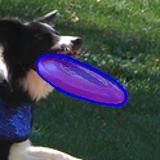
\includegraphics[width=2.4cm]{images/coco/00893.jpg}}          \hspace{-0.6em}        
    \subfloat{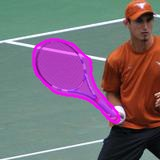
\includegraphics[width=2.4cm]{images/coco/01107.jpg}}          \hspace{-0.6em}        
    \subfloat{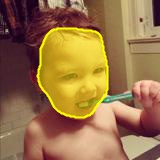
\includegraphics[width=2.4cm]{images/coco/01108.jpg}}          \hspace{-0.6em}        
    \subfloat{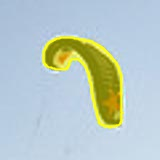
\includegraphics[width=2.4cm]{images/coco/01564.jpg}}          \hspace{-0.6em}        
    \subfloat{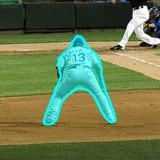
\includegraphics[width=2.4cm]{images/coco/01664.jpg}}\\[0.2ex]
    \subfloat{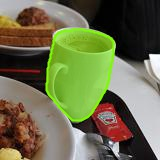
\includegraphics[width=2.4cm]{images/coco/01939.jpg}}                     \hspace{-0.6em}
    \subfloat{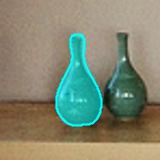
\includegraphics[width=2.4cm]{images/coco/02078.jpg}}                     \hspace{-0.6em}
    \subfloat{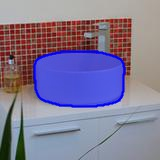
\includegraphics[width=2.4cm]{images/coco/02285.jpg}}                     \hspace{-0.6em}
    \subfloat{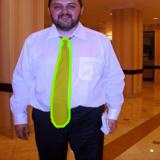
\includegraphics[width=2.4cm]{images/coco/02497.jpg}}                     \hspace{-0.6em}
    \subfloat{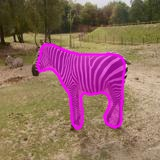
\includegraphics[width=2.4cm]{images/coco/02589.jpg}}\\[0.2ex]
    \subfloat{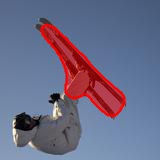
\includegraphics[width=2.4cm]{images/coco/02700.jpg}}                   \hspace{-0.6em}
    \subfloat{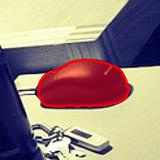
\includegraphics[width=2.4cm]{images/coco/03000.jpg}}                   \hspace{-0.6em}
    \subfloat{
\includegraphics[width=2.4cm]{images/coco/03327.jpg}}                   \hspace{-0.6em}
    \subfloat{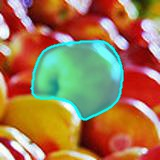
\includegraphics[width=2.4cm]{images/coco/03482.jpg}}                   \hspace{-0.6em}
    \subfloat{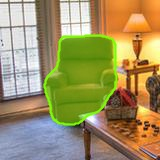
\includegraphics[width=2.4cm]{images/coco/03733.jpg}}
    \caption{Segmentation results of InstMask on COCO2017 \cite{Lin2014MicrosoftCC} validation dataset.}
    \label{fig:InstMask}
\end{figure}

In this work, we propose the Instance Guided Correlation Filter (IGCF) to address the aforementioned limitations. Specifically, a deep network, namely InstMask, is designed to generate accurate instance masks of targets. InstMask is trained off-line and end-to-end, using a data-driven approach, to learn semantic information from the segmentation training sets, e.g. those in COCO2017\cite{Lin2014MicrosoftCC} (see Fig. \ref{fig:InstMask}). The instance mask can facilitate the learning of the correlation filters by enabling the removal of background clutter from the training images that contain targets. 

Unlike common object segmentation tasks, we have designed a new network structure and training method that enables InstMask to identify salient objects of arbitrary category located near the center of a search patch. InstMask is not restricted to identifying targets in categories that appear in the training set. Moreover, our network embodied with one $1 \times 1$ convolution layer allows a global receptive field to obtain contextual information from the neighbourhood of the target. This increases the accuracy of the segmentation. This lightweight network achieves a balance between tracking accuracy and speed while running at 5 FPS on a single CPU core platform. 

The correlation filters are updated online in order to adapt to particular targets. In contrast, InstMask is non-adaptive. These two sources of information about the track are complementary. They can be combined to further improve the robustness demand are independent and complementary. So the outputs of the two components can be integrated together to further improve the tracking performance. We further propose a self-correction mechanism to mitigate the drift problem of CF trackers. The geometric center of the segmentation mask is used to correct the prediction bias of the correlation filters. Equipped with the InstMask module, the proposed IGCF not only tracks targets accurately, but it can also be used for video object segmentation. This demonstrates the wide range of applications of our algorithm. The architecture of the proposed tracking framework IGCF is shown in Fig. \ref{fig:IGCF}.

\begin{figure*}
    \centering
    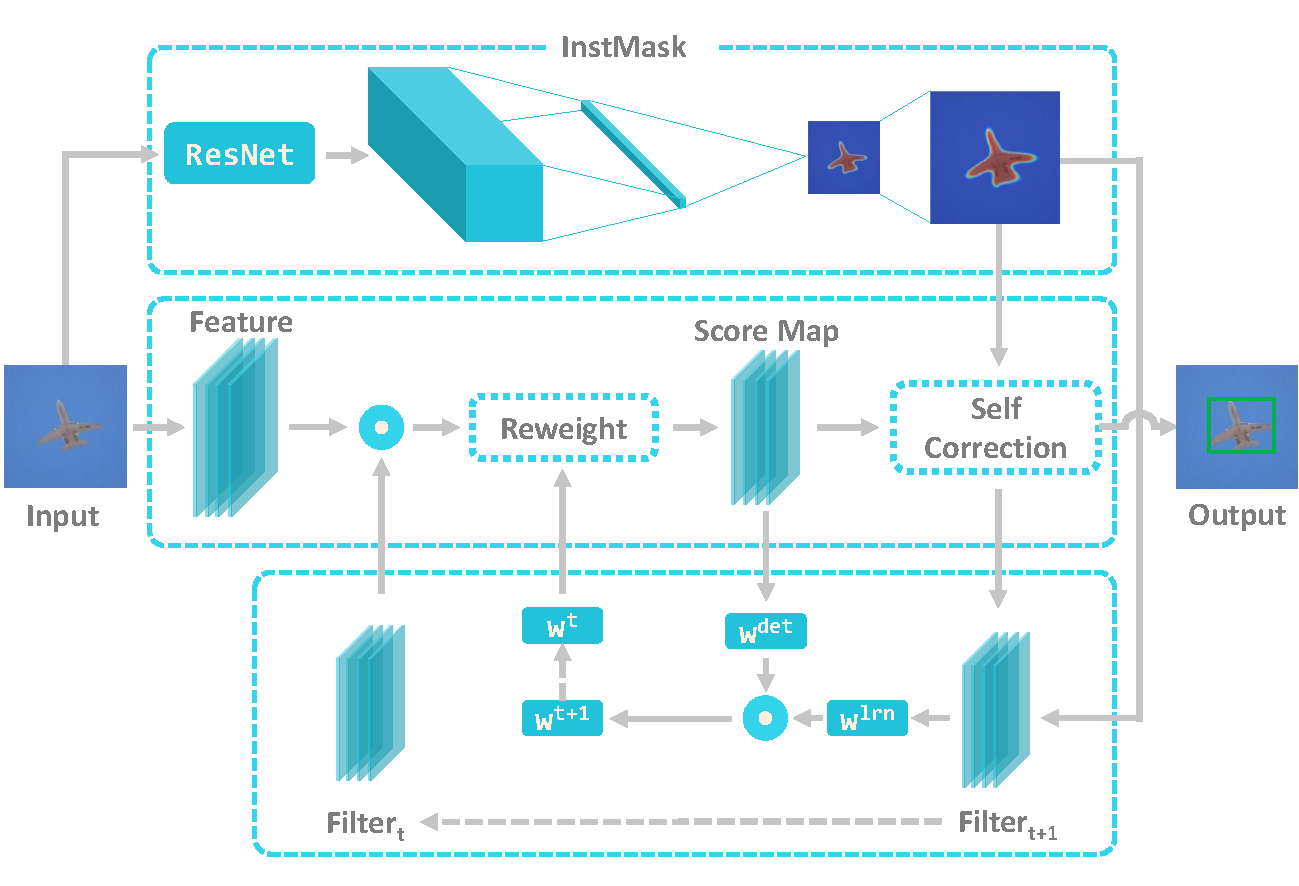
\includegraphics[width=12cm]{images/instmask1.pdf}
    \caption{Architecture of the tracking framework IGCF.}
    \label{fig:IGCF}
\end{figure*}

We performed comprehensive experiments on three tracking benchmarks: VOT2015 \cite{Kristan2015TheVO}, VOT2016 \cite{Kristan2016TheVO} and GOT-10K \cite{Huang2018GOT10kAL}. Our IGCF tracker performs favorably against state-of-the-art trackers while achieving a good balance between tracking accuracy. Finally, we performed qualitative experiments on the video object segmentation dataset DAVIS2016 \cite{Perazzi2016}, in order to show the powerful video semantic segmentation and tracking capabilities of our algorithm.

\section{Related works}
Object tracking has been a popular topic for decades. The goal of object tracking is to establish the positions of a target in the frames of a video, given the position of the target in the first frame.

\subsection{DCF-based trackers}
Many DCF based target trackers are designed to take account of partial occlusion, illumination variation, background clutter, motion blur, viewpoint change, etc.

Bolme et al. proposed a tracker \cite{Bolme2010VisualOT} based on Minimum Output Sum of Squared Error (MOSSE) filters. The tracker is robust to variations in lighting, scale, pose, and non-rigid deformations while operating at 669 frames per second.
The CSK tracker \cite{Henriques2012ExploitingTC} improves on the MOSSE tracker by adopting the circulant structure of subwindows of an image, and using the Fast Fourier Transform (FFT) to quickly incorporate information from all subwindows. Additionally, it is shown in \cite{Henriques2012ExploitingTC} that classification in non-linear spaces can be done as efficiently as in the original image space using the kernel trick.
Danelljan et al. \cite{Danelljan2014AdaptiveCA} improve the CSK tracker by learning multi-channel filters on multi-dimensional color attributes. To avoid the computational overhead caused by the high dimensions of the color attributes, an adaptive dimension reduction technique is proposed \cite{Danelljan2014AdaptiveCA} to reduce the original eleven dimensions to only two.
Later on, Henriques et al. \cite{Henriques2015HighSpeedTW} propose an analytic model for datasets of thousands of translated patches. The model is diagonalized using the Discrete Fourier Transform. This operation can reduce both storage and computation by several orders of magnitude.

Recently, many studies \cite{Danelljan2015LearningSR, Lukezic2017DiscriminativeCF} have introduced spatial constraints into the learning of correlation filters. A tracker called Spatially Regularized Discriminative Correlation Filters (SRDCF) is proposed in \cite{Danelljan2015LearningSR}. The SRDCF introduces a spatial regularization component in the learning to penalize correlation filter coefficients depending on their spatial location.
Moreover, the CSR-DCF filter described in \cite{Lukezic2017DiscriminativeCF} introduces the channel and spatial reliability components to DCF tracking and provides a learning algorithm for their efficient and seamless integration in the filter update and tracking processes. The spatial reliability component adjusts the filter support to a suitable part of the target. The channel reliability component generates feature weighting coefficients, depending on the locations of the features. The CSR-DCF tracker has a large search region and tracks non-rectangular targets effectively. The spatial reliability component bears some similarities to the pixel-wise learner with color distribution used in the Staple (Sum of Template And Pixel-wise LEarners) \cite{Bertinetto2016StapleC} tracker. This tracker combines complementary cues to improve robustness. It solves two independent ridge-regression problems with respect to the CF-based template model and pixel-wise color distribution model.

In order to handle the scale changes of a target, the method proposed in \cite{Li2014ASA} samples the target at different scales, and adjusts the samples into a fixed size for matching with the learnt model at each frame. This method also adopts a multiple feature integration scheme, which employs the raw pixel, Histogram of Gradients \cite{Forsyth2014ObjectDW} and color-naming \cite{Weijer2009LearningCN} to further enhance the tracker.

\subsection{CNN-based trackers}
In the past few years, deep learning \cite{Goodfellow2015DeepL} has achieved remarkable success in many research fields, especially in computer vision \cite{Girshick2016RegionBasedCN, Schroff2015FaceNetAU}, speech recognition \cite{Kim2016JointCB, Wu2015DeepNN} and natural language processing \cite{Vinyals2014GrammarAA, Bahdanau2014NeuralMT}. Several trackers have demonstrated the performance advantages of deep learning. 

Most DCF-based trackers are restricted to single-resolution feature maps, significantly limiting their potential. To solve this problem, the CCOT tracker \cite{Danelljan2016BeyondCF} learns continuous convolution filters to fuse the feature maps obtained at different resolutions. This produces a continuous-domain confidence map for the target. In addition to multi-resolution fusion, the continuous domain learning formulation enables accurate sub-pixel localization.
The ECO tracker \cite{Danelljan2016ECOEC} includes in the core DCF formulation a factorized convolution operator, a compact generative model of the training sample distribution and a conservative model update strategy. This alleviates the computational overhead due to the use of CNN features. In contrast, the CF2 tracker \cite{Ma2015HierarchicalCF} adaptively learns correlation filters on each convolutional layer to encode the target appearance and infers the target location using the correlation response of each layer.

Held et al. \cite{held2016learning} propose an off-line trained neural network to track targets at 100 fps on a GPU platform. They use a simple feed-forward network without online training. The network learns a generic relationship between object motion and appearance and can be used to track novel objects that do not appear in the training set. 
Recently, a series of trackers such as SiamFC \cite{bertinetto2016fully}, SiamRPN \cite{Li2018HighPV}, DasiamRPN \cite{zhu2018distractor} and SiamMask \cite{Wang2018SiamMask}, use a siamese network to learn the similarity between search images and exemplar images. They obtain a good balance between tracking speed and accuracy. SiamMask is the first attempt to perform both tracking and segmentation simultaneously in one end-to-end learning framework.

Despite attractive performances both in accuracy and robustness, most of the above trackers only exploit features extracted from deep convolutional neural networks. There is a lack of semantic information semantic information at the instance level. Moreover, they have a high computational overhead for feature extraction, and thus are not suitable for low-cost platforms. For example, the SiamMask algorithm runs only at 1 FPS on the Intel E5-2620 CPU platform.

There are also some works dedicated to improving tracking robustness using a self-correction mechanism to mitigate the tracking drift. For instance in \cite{fan2017parallel}, the tracking framework consists of two components, a tracker and a verifier, working in parallel on two separate threads. The tracker provides real-time tracking inference and is expected to perform well most of the time. In contrast, the verifier checks the tracking results and corrects the tracker when needed.

\section{The Proposed Method}

\subsection{Tracking Formulation} \label{sec:InstMask}
DCF trackers \cite{Bolme2010VisualOT, Danelljan2014AccurateSE, Henriques2015HighSpeedTW, Li2014ASA} have been widely studied and used. Specifically, consider the appearance feature: $f=\{f_d\}_{d=1:N_c}$ of an target, where $N_c$ is the channel number of the target feature. The goal of DCF-like trackers is to train a filter $h=\{h_d\}_{d=1:N_c}$, such that the correlation response between the feature and the filter fits the desired output $g$ which is typically a 2-D Gaussian function centered at the target location: 
\begin{equation} \label{eq:dcf}
\tilde{g}=\sum_{d=1}^{N_c}f_d \star h_d \cdot w_d,
\end{equation}
where $\star$ represents the circular correlation operator and channel weights $w = \{w_d\}_{d=1:N_c}$ are the scaling factors based on the discriminative power of each feature channel \cite{Lukezic2017DiscriminativeCF}.
The position of the peak of the response map is the estimated position of the target in the current frame.
The optimal correlation filter $h$ is estimated by minimizing:
\begin{equation}
\varepsilon(h) = \sum_{d=1}^{N_c}||f_d \star h_d - g||^2+\lambda||h_d||^2.
\end{equation}

Recently, many studies \cite{Danelljan2015LearningSR, Lukezic2017DiscriminativeCF, Galoogahi2017LearningBC, Xu2018LearningAD, Feng2018LearningSR} have demonstrated that spatial constraints imposed on a target improve the correlation filter learning by reducing the background interference. As described in \cite{Lukezic2017DiscriminativeCF}, the segmentation mask of an image patch is a spatial map with elements either 1 or 0, that indicate whether pixels belong to the target or belong to the background. During the filter training process, the filter $h$ is constrained by the mask $m$: $h \equiv m \odot h$, where $\odot$ represents the Hadamard (element-wise) product. This constraint adapts the filter support to the part of the target suitable for tracking. This makes it possible to use a large training region to capture more context information and overcomes the limitations of the rectangular boxes.

\subsection{InstMask}
Recently, many studies \cite{Danelljan2015LearningSR, Lukezic2017DiscriminativeCF, Galoogahi2017LearningBC, Xu2018LearningAD, Feng2018LearningSR} have introduced spatial constraints into the learning of correlation filters with good results. In this paper we use segmentation masks of tracked targets to learn better correlation filters. For efficiency and performance reasons, an ideal segmentation method should possess three key characteristics: (1) seamless integration with the tracking process, (2) be simple enough to accommodate the speed requirement of tracking, and (3) the proposed segment should match the target as accurately as possible.
Most previous approaches for generating spatial constraints, rely on hand-designed rules or low-level image features like color histograms.
In this paper, we present the InstMask network, which generates acute instance masks for targets. InstMask is trained off-line and end-to-end using the data-driven approach to learn semantic information from the segmentation training sets, such as those in COCO2017 \cite{Lin2014MicrosoftCC}. The instance mask can constrain the learning of the correlation filters by suppressing background clutter in the positive samples. Based on the instance-level segmentation, we further propose a self-correction mechanism to mitigate the drift problem of CF trackers. This approach provides a notable gain in object tracking accuracy compared to classic DCF approaches.
Unlike previous approaches for generating segmentation masks, we do not rely on edges, superpixels, or any other form of low-level segmentation. Instead, the core of our model is a ConvNet. By leveraging powerful ConvNet feature representations trained on ImageNet and adapted on the large amount of segmented training data available in COCO, we are able to generate semantic segmentation masks for targets to constrain the learning of correlation trackers.
It is worth noting that it is sub-optimal to integrate the existing instance segmentation methods to provide spatial constraints for correlation filter learning. General tracking algorithms usually have complex network structures, which make it hard to strike a balance between tracking accuracy and speed. In contrast, the segmentation network proposed in this paper is designed for tracking and is lightweight, running at 5 FPS on the CPU.

When tracking in the $i$-th frame, the segmentation mask of the target in frame $i$ needs to be obtained to constrain the learning of the correlation filter. Since the tracker has generated $p_{i-1}$, i.e., the position of the target in frame $i-1$, and the displacement of the target in two adjacent frames is small, we can crop the small image patch in frame $i$ centered on $p_{i-1}$ and send the patch to InstMask to get the segmentation mask.
During tracking, the target position is assumed to be in the vicinity of the target position in the previous frame.
This design has the following advantages: (1) Because of the strong consistency of the input data, the network can obtain accurate segmentation results using fewer parameters. (2) Because the network has fewer parameters and the image patch is small, only a short time is required for inference. (3) Searching around the target's previous location can avoid the adverse effects of distractors located in the background. During training, each sample $k$ in the training set contains (1) the RGB input patch $x_k$, which contains a target near to the centre of the input patch, (2) the binary mask $m_{k}$ corresponding to the input patch.
We next describe the architecture and the training procedure.

\textbf{Architecture} The network architecture is shown in Table \ref{tab:InstMask} and Fig. \ref{fig:net}. The backbone of InstMask is constructed based on ResNet50 \cite{He2016DeepRL}, which consists of a stem block and 3 residual blocks.
The input to InstMask is a 160$\times$160$\times$3 image patch. It is sent to the stem block, producing a 80$\times$80$\times$64 feature map. Then the feature map is sent to 3 residual blocks sequentially, producing feature maps of size 40$\times$40$\times$256, 20$\times$20$\times$512, 10$\times$10$\times$1024, respectively. Subsequently, the obtained feature map is sent to three convolution layers to generate the vector of length 3136, which allows a global receptive field to perceive all of the contextual information about the target. Finally, this vector is reshaped to 56$\times$56 to get the final segmentation mask. Since it is such a lightweight network, our proposed tracking method optimally balances the tracking accuracy and speed while running at 5 FPS on the platform with a Intel E5-2620 CPU core, making it possible to deploy the tracker in real-world applications including autonomous driving, robotics and augmented reality.

\iffalse
\begin{algorithm}
  \caption{The IGCF tracking algorithm.} 
  \begin{algorithmic}
    \Require Image $I_t$, object position on previous frame $p_{t-1}$, scale $s_{t-1}$, filter $h_{t-1}$, channel reliability $w_{t-1}$.
    \Ensure Position $p_t$, scale $s_t$ and updated models.
  \Statex
  \LState \textbf{Localization:}
  \begin{enumerate}[leftmargin=0pt,itemindent=1.5em]
    \item $p_t$: position of the maximum in correlation between $h_{t-1}$ and image patch features $f_{t}$ extracted on position $p_{t-1}$ and weighted by the channel reliability scores $w_{t-1}$ (Eq. \ref{eq:dcf}).
    \item Estimate segmentation mask $m$ (Sect. \ref{sec:InstMask}).
    \item Correct $p_t$ using $m$ (Sect. \ref{sec:cog}).
    \item Using location $p_t$, estimate new scale $s_ t$ as in \cite{Danelljan2014AccurateSE}.
    \item Estimate detection reliability $\tilde{w}^{(det)}$  from per-channel responses using (\ref{eq:det}).
  \end{enumerate}
  \LState \textbf{Update:}
  \begin{enumerate}[leftmargin=0pt,itemindent=1.5em]
    \item Estimate a new filter $\tilde{h}$ from $m$ using (\ref{eq:h1})$\sim$(\ref{eq:h3}).
    \item Estimate learning channel reliability $\tilde{w}^{(lrn)}$ from $h$ using (\ref{eq:lrn}).
    \item Calculate channel reliability $\tilde{w}$ using (\ref{eq:c}).
    \item Update filter $h_t$ and channel reliability $w_t$ using (\ref{eq:update1}) and (\ref{eq:update2}).
  \end{enumerate}
\end{algorithmic}
\end{algorithm}
\fi

\textbf{Training} During training, the 56$\times$56 mask is up-sampling to the original image size 160$\times$160. Let $l$ denotes pixel-wise ground-truth mask of size $w \times h$. The loss is calculated as:
\begin{equation}
L = \frac{1}{wh} \sum_{xy}{log(1+e^{-l_{x,y}P_{x,y}})},
\end{equation}
where $l_{x,y} \in \{ \pm 1 \}$ is the label corresponding to pixel $(x,y)$ of the object mask, and $P_{x,y}$ is the prediction of InstMask at location $(x,y)$.

The COCO2017 \cite{Lin2014MicrosoftCC} instance segmentation dataset is used to train InstMask.
Contrast with many segmentation networks which only predict categories that appear in the training set, the proposed InstMask ignores category information during training and works as a class-agnostic segmentation network. In effect, InstMask detects salient targets in the search region. Although InstMask uses COCO dataset \cite{Lin2014MicrosoftCC} with only 80 classes for training, the network is able to segment targets in categories that do not appear in the training set, as shown in Fig. \ref{fig:IGSC}.
We train our model using stochastic gradient descent with a batch size of 32 examples, momentum of 0.9, and weight decay of 0.00005. There are totally 50 epoches. The learning rate is decreased in log space from $10^{-2}$ to $10^{-4}$. During training, the input image size is set to 160$\times$160, and the target is located at the center of the image, with a size of 112$\times$112. To enhance the generalization of the network, we perform data augmentation. Specifically, we consider translation shifts (of $\pm$16 pixels), scale deformations (of $2^{\pm 1/4}$), and also horizontal flips.

InstMask is trained offline. During the tracking InstMask only carries out a forward propagation process without the back propagation of the gradient. This not only prevents drift, but also meets the real-time requirements of tracking.

Although our model shares high level similarities with CSRDCF \cite{Lukezic2017DiscriminativeCF}, the principle of the implementation is very different.
In CSRDCF \cite{Lukezic2017DiscriminativeCF}, the segmentation masks are generated using the color histograms of the target and background. This heuristic approach has several disadvantages: (1) Since only low-level pixel information is used, it is difficult to accurately segment an target. (2) In order to adapt to the apparent changes of the target, the histogram model is constantly updated during the tracking process, which easily leads to drift of the tracker. In contrast, InstMask does not update the colour histogram online. This improves computational efficiency while avoiding the undesired drift. Besides, tracking results are more accurate because of the use of semantic level rather than pixel-level information for segmentation.

\setlength\extrarowheight{1pt}
\begin{table}
\centering
\caption{Network design of InstMask.}
\begin{tabular}{|c|c|c|}
\hline
Layers & Output Size & Support \\\hline
Data & $160 \times 160 \times 3$ &  -\\\hline
Stem Block & $80 \times 80 \times 64$ &  $ 7 \times 7 \text{ conv} $\\\hline
\multirow{4}*{Res Block (1)} & $40 \times 40 \times 64$ &  $ 2 \times 2 \text{ maxpool} $\\\cline{2-3}
~ & $40 \times 40 \times 256$ &  $ \left [ \begin{array}{l} 1 \times 1 \text{ conv} \\ 3 \times 3 \text{ conv} \\ 1 \times 1 \text{ conv} \end{array} \right ] \times 3 $\\\hline
Res Block (2) & $20 \times 20 \times 512$ &  $ \left [ \begin{array}{l} 1 \times 1 \text{ conv} \\ 3 \times 3 \text{ conv} \\ 1 \times 1 \text{ conv} \end{array} \right ] \times 4 $\\\hline
Res Block (3) & $10 \times 10 \times 1024$ &  $ \left [ \begin{array}{l} 1 \times 1 \text{ conv} \\ 3 \times 3 \text{ conv} \\ 1 \times 1 \text{ conv} \end{array} \right ] \times 6 $\\\hline
\multirow{5}*{Decoder} & $10 \times 10 \times 128$ &  $ 1 \times 1 \text{ conv} $\\\cline{2-3}
~ & $1 \times 1 \times 512$ &  $ 10 \times 10 \text{ conv} $\\\cline{2-3}
~ & $1 \times 1 \times 3136$ &  $ 1 \times 1 \text{ conv} $\\\cline{2-3}
~ & $56 \times 56$ & reshape \\\cline{2-3}
~ & $160 \times 160$ & upscale \\\hline
\end{tabular}
\label{tab:InstMask}
\end{table}

\begin{figure*}
    \centering
    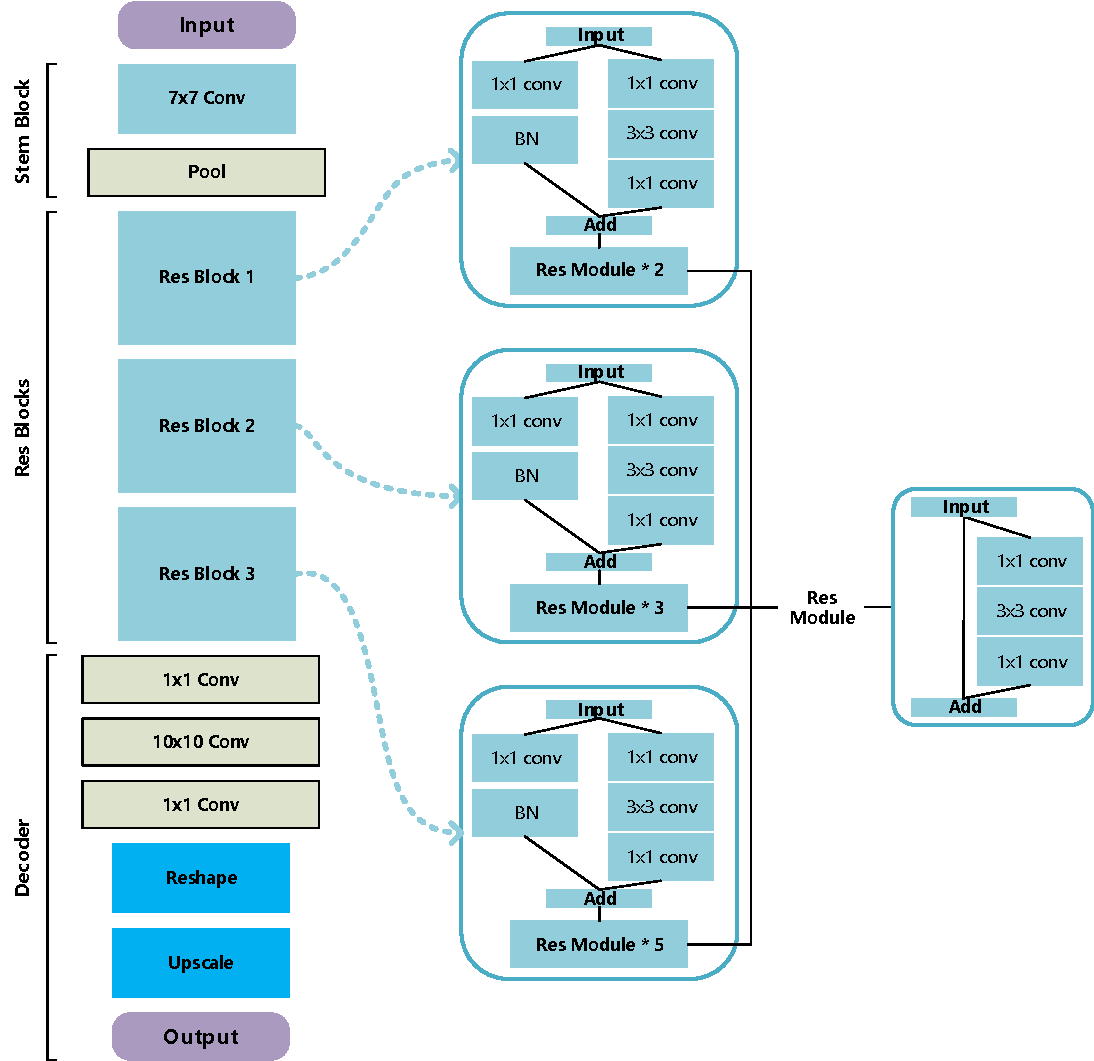
\includegraphics[width=12cm]{images/net.pdf}
    \caption{Architecture of our InstMask.}
    \label{fig:net}
\end{figure*}

\subsection{Instance Guided Self-Correction Component} \label{sec:cog}
InstMask allows better filters to be learnt and it helps to correct poor tracking results. The result of the DCF is generated by the ground truth position of the target in the first frame, and the following predicted target positions. InstMask is trained by COCO \cite{Lin2014MicrosoftCC}, and acts as a universal salient object detector, which recognizes the object at the centre of the image. During tracking, InstMask does not need any information about ground truth or the predicted target positions in the following frames. Therefore, the correlation filters that adapt on-line to a particular target and the static InstMask to make the tracking robust are complementary. The outputs of the two components can be integrated together to further improve the tracking performance. In this subsection, we present a method to integrate the DCF result and the InstMask result, to make a more stable tracker.

In the DCF module, the position of the maximum of the correlation between filter $h$ and feature $f$ is regarded as the target position in the current frame. However, because of the on-line updating, the correlation filters can easily drift.

The result of InstMask also gives some information about the location of the target. During tracking, the current image frame is cropped away from the target position in the previous frame. The displacement of a target between two frames is usually small, so the target in the current frame is often near the center of the cropped image patch and can be recognized by InstMask. However, we cannot rely only on the InstMask to produce the final tracking result because InstMask is not updated on-line.

To utilize the advantages of both results and overcome their shortcomings, we propose the \textbf{I}nstance \textbf{G}uided \textbf{S}elf-\textbf{C}orrection component IGSC. IGSC combines both results, to obtain a better track. Specifically, the mask $m$ is generated according to $P$ using the hard threshold $b \in [0, 1] $:
\begin{equation}
m_{x,y} = \left\{ \begin{array}{ll}
 1 & \textrm{if $P_{x,y} > b$}\\
 0 & \textrm{if $P_{x,y} \le b$}
 \end{array} \right.
\end{equation}
$P$ is the probability map generated from InstMask. The element $P_{x,y}$ is the probability that a pixel $(x,y)$ belongs to the target.
Then the target position is obtained from $m$:
\begin{equation}
c_{m} = Centroid(m).
\end{equation}
The self correction process can be described as following:
\begin{equation}
p = \left\{ \begin{array}{ll}
 c_{m} & \textrm{if $||c_{m}-c_{dcf}||_2^2 < \beta$}\\
 c_{dcf} + \alpha \cdot (c_{m}-c_{dcf}) & \textrm{otherwise}
 \end{array} \right.,
\end{equation}
where $c_{dcf}$ is the position predicted by DCF, $\alpha$ is a hyper-parameter to control the strength of the self-correction, and $\beta$ is a threshold on the distance between $c_{m}$ and $c_{dcf}$.
Thanks to the robustness of the segmentation results, the tracker can correct itself when the DCF result shows an unstable drift. The effectiveness of the proposed instance guided self-correction component is shown in Fig. \ref{fig:IGSC}.

\begin{figure} 
    \subfloat{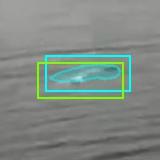
\includegraphics[width=2.45cm]{images/cog/birds1/00003.jpg}}          \hspace{-0.6em}        
    \subfloat{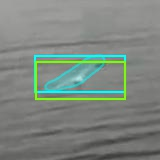
\includegraphics[width=2.45cm]{images/cog/birds1/00005.jpg}}          \hspace{-0.6em}        
    \subfloat{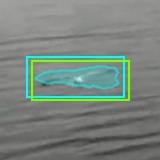
\includegraphics[width=2.45cm]{images/cog/birds1/00007.jpg}}          \hspace{-0.6em}        
    \subfloat{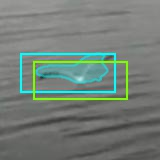
\includegraphics[width=2.45cm]{images/cog/birds1/00013.jpg}}          \hspace{-0.6em}        
    \subfloat{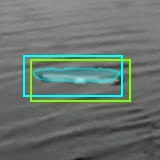
\includegraphics[width=2.45cm]{images/cog/birds1/00057.jpg}}\\[0.2ex]
    \subfloat{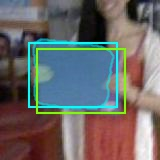
\includegraphics[width=2.45cm]{images/cog/book/00002.jpg}}                     \hspace{-0.6em}
    \subfloat{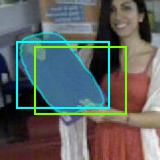
\includegraphics[width=2.45cm]{images/cog/book/00005.jpg}}                     \hspace{-0.6em}
    \subfloat{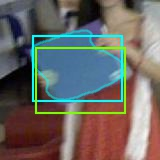
\includegraphics[width=2.45cm]{images/cog/book/00011.jpg}}                     \hspace{-0.6em}
    \subfloat{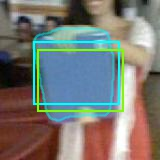
\includegraphics[width=2.45cm]{images/cog/book/00013.jpg}}                     \hspace{-0.6em}    \subfloat{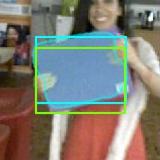
\includegraphics[width=2.45cm]{images/cog/book/00016.jpg}}\\[0.2ex]
    \subfloat{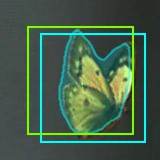
\includegraphics[width=2.45cm]{images/cog/butterfly/00015.jpg}}                   \hspace{-0.6em}
    \subfloat{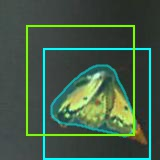
\includegraphics[width=2.45cm]{images/cog/butterfly/00019.jpg}}                   \hspace{-0.6em}
    \subfloat{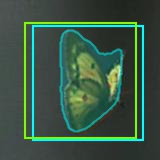
\includegraphics[width=2.45cm]{images/cog/butterfly/00025.jpg}}                   \hspace{-0.6em}
    \subfloat{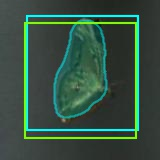
\includegraphics[width=2.45cm]{images/cog/butterfly/00027.jpg}}                   \hspace{-0.6em}
    \subfloat{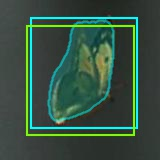
\includegraphics[width=2.45cm]{images/cog/butterfly/00031.jpg}}
    \caption{The tracking result before (green) and after (blue) the instance guided self-correction component.}
    \label{fig:IGSC}
\end{figure}

\subsection{Overview}
The tracking process consists of two phases: localization and model update. 
At the localization phase, the target position $p_t$ is the position of the maximum in correlation between $h_{t-1}$ and image patch features $f$ extracted from the position $p_{t-1}$ and weighted by the channel reliability scores $w$ (Eq. \ref{eq:dcf}).
The segmentation mask $m$ is estimated using the proposed InstMask network (Sect. \ref{sec:InstMask}).
The centroid of the segmentation mask is used to correct the prediction bias of the correlation filter (Sect. \ref{sec:cog}).
Then the new scale $s_t$ is estimated by a single scale-space correlation filter as in \cite{Danelljan2014AccurateSE}.
The channel detection reliability $\tilde{w}^{(det)}$ is estimated as follows \cite{Lukezic2017DiscriminativeCF}:
\begin{equation} \label{eq:det}
\tilde w_d^{(det)} = max(1 - \rho_d^{max2} / \rho_d^{max1}, 0.5),
\end{equation}
which reflects how uniquely each channel votes for a single target location. The $\tilde w_d^{(det)}$ are used to calculate $w$ later (Eq. \ref{eq:c}). $\rho_d^{max2}$ and $\rho_d^{max1}$ are the second and first highest non-adjacent peaks in the correlation response of channel $d$, respectively.

At the model update phase, the new filter $\tilde{h}$ is estimated using mask $m$. We use the iterative approach proposed in \cite{Lukezic2017DiscriminativeCF} for efficiently solving the filter. Let $l$ be the Lagrange multiplier, $\mu > 0$, $h_m=m \odot h$, $\hat{h}^0 = h_{t-1}$ and $\hat{l}^0 = 0$. In each iteration, the following sub-problems are solved sequentially as in \cite{Lukezic2017DiscriminativeCF}:
\begin{equation} \label{eq:h1}
\hat{h}_c^{i+1} = \frac{\hat{f} \odot \bar{\hat{g}} +(\mu^i \hat{h}_m^i - \hat{l}^i)}{\bar{\hat{f}} \odot \hat f + \mu^i}
\end{equation}
\begin{equation}
h^{i+1} = \frac{m \odot \mathcal{F}^{-1}[\hat{l}^i + \mu^i\hat{h}_c^{i+1}]}{\frac{\lambda}{2D} + \mu^i}
\end{equation}
\begin{equation} \label{eq:h3}
\hat{l}^{i+1} = \hat{l}^i + \mu(\hat{h}_c^{i+1} - \hat{h}^{i+1})
\end{equation}
Then the channel reliability $\tilde w_d$ \cite{Lukezic2017DiscriminativeCF} consisting of the channel learning reliability $\tilde w_d^{(lrn)}$ and the channel detection reliability $\tilde w_d^{(det)}$ is calculated as follows: 
\begin{equation} \label{eq:c}
\tilde w_d = \tilde w_d^{(lrn)} \cdot \tilde w_d^{(det)},
\end{equation}
where $\tilde{w}^{(lrn)}$ is represents the maximum response value of a learned channel filter:
\begin{equation} \label{eq:lrn}
\tilde{w}_d^{lrn} = max(f_d * h_d).
\end{equation}
Finally, the filter and channel reliability are updated online:
\begin{equation} \label{eq:update1}
h_t = (1 - \eta)h_{t-1} + \eta \tilde{h}
\end{equation}
\begin{equation} \label{eq:update2}
w_t = (1-\eta)w_{t-1} + \eta \tilde{w},
\end{equation}
where $\eta$ is the learning rate used to control the speed of model update.

\begin{figure}
    \centering
    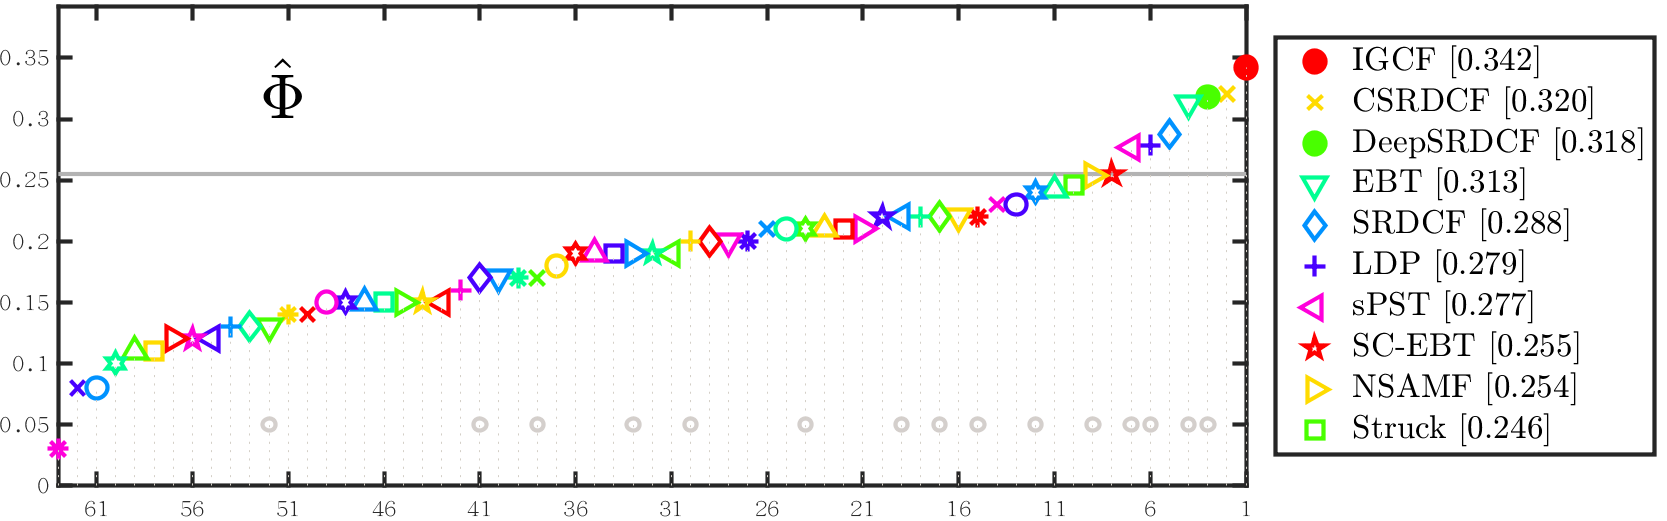
\includegraphics[width=12cm]{images/vot/eao_rank_vot2015.png}
    \caption{Expected average overlap (EAO) plot on VOT2015 \cite{Kristan2015TheVO}.}
    \label{fig:vot15}
\end{figure}

\begin{figure}
    \centering
    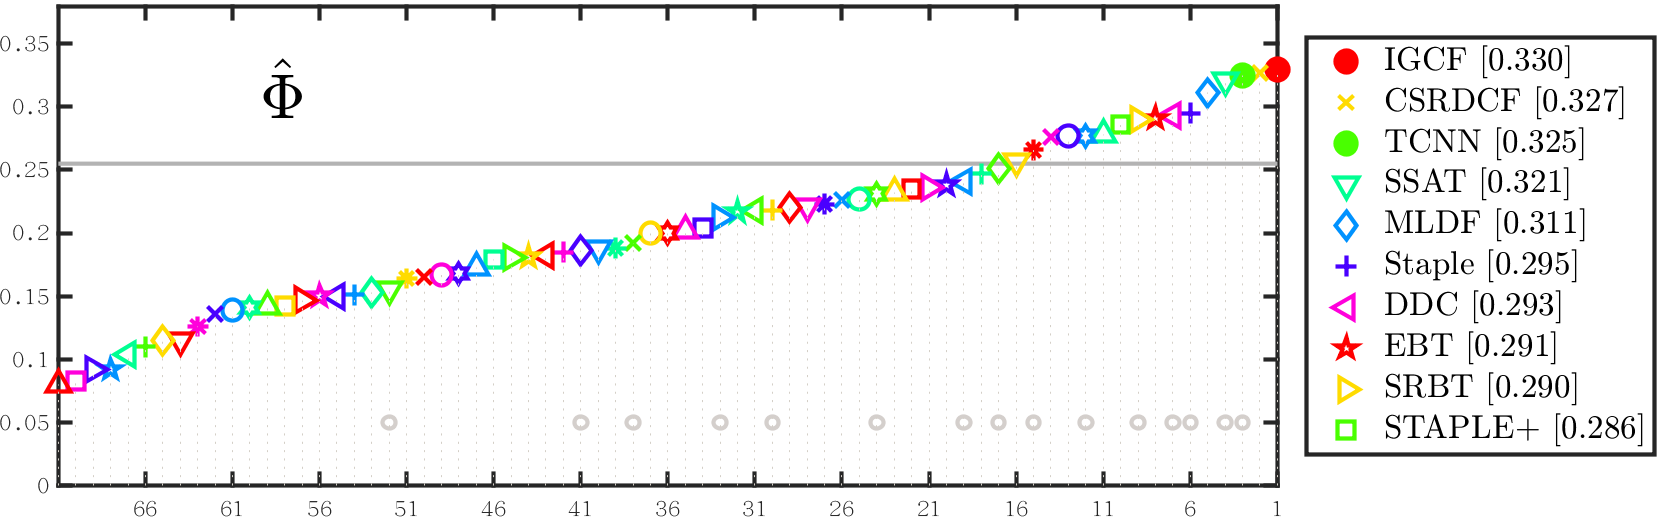
\includegraphics[width=12cm]{images/vot/eao_rank_vot2016.png}
    \caption{Expected average overlap (EAO) plot on VOT2016 \cite{Kristan2016TheVO}.}
    \label{fig:vot16}
\end{figure}

\section{Experiments}
We provide a comprehensive evaluation of the proposed tracker IGCF on three challenging object tracking datasets: VOT2015 \cite{Kristan2015TheVO}, VOT2016 \cite{Kristan2016TheVO} and GOT-10K \cite{Huang2018GOT10kAL}. Note that there is no overlap between the videos used for training the InstMask component and the evaluation datasets. In addition, a qualitative experiment is carried out on the video object segmentation dataset DAVIS \cite{Perazzi2016}.
\subsection{Evaluation on VOT2015}

\begin{figure}
    \centering
    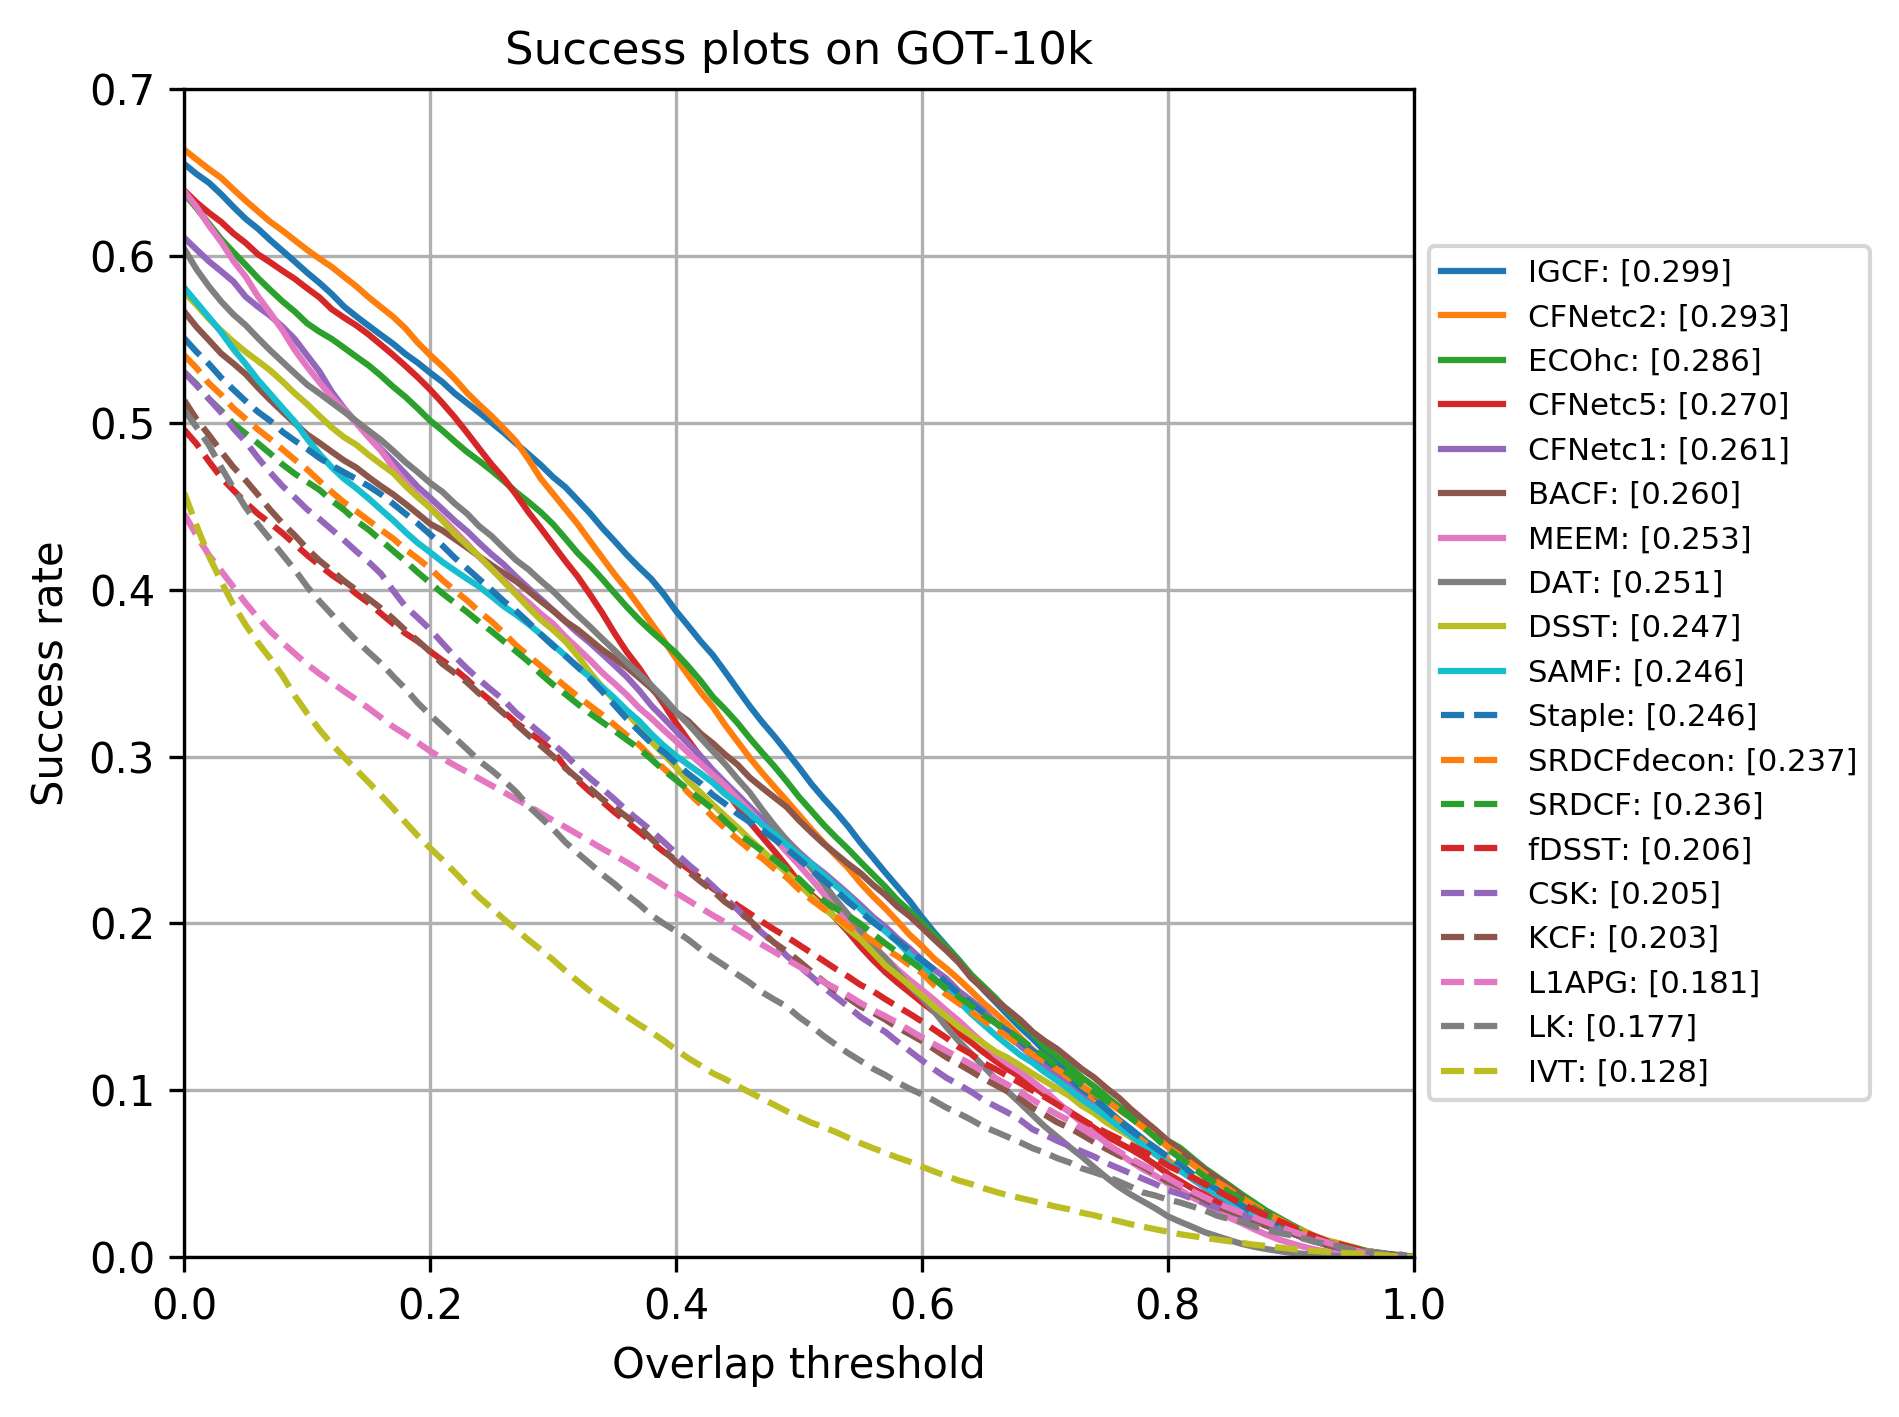
\includegraphics[width=12cm]{images/got10k/success_plot.png}
    \caption{Overall performance on GOT-10k \cite{Huang2018GOT10kAL}, ranked by their average overlap (AO) scores.}
    \label{fig:got10k}
\end{figure}

The VOT2015 \cite{Kristan2015TheVO} tracking dataset contains 60 challenging videos. It is constructed from over 300 sequences by an advanced sequence selection methodology that favours targets difficult to track and maximizes a visual attribute diversity cost function. 
In VOT2015, three metrics are used to evaluate the performance of a tracker: (1) accuracy, (2) robustness and (3) EAO (expected average overlap). The accuracy measures how well the bounding box predicted by the tracker overlaps with the ground truth bounding box. The robustness measures how many times the tracker loses the target (fails) during tracking. EAO combines accuracy and robustness to evaluate the overall performance of the tracker. 

We compare our algorithm with the following trackers: CSRDCF \cite{Lukezic2017DiscriminativeCF}, SRDCF \cite{Danelljan2015LearningSR}, TGPRfSRDCF \cite{gao2018tracking}, DeepSRDCF \cite{Danelljan2015ConvolutionalFF}, TCNN \cite{nam2016modeling}, Staple \cite{Bertinetto2016StapleC}, EBT \cite{Zhu2016BeyondLS}, NSAMF \cite{Hua2015OnlineOT} and Struck \cite{Hare2011StruckSO}.
These trackers can be classified into three categories: Struck and EBT are traditional trackers. SRDCF, CSRDCF, TGPRfSRDCF, Staple and SAMF are DCF-based trackers. DeepSRDCF and TCNN are CNN-based trackers.
The EAO scores of the trackers are shown in Fig. \ref{fig:vot15}. Compared to other listed approaches, our approach achieves a superior EAO of 0.342. 
Struck uses a kernelized structured output support vector machine (SVM), which is learned online to provide adaptive tracking. In contrast, IGCF is based on powerful correlation filters. As a result, IGCF significantly outperforms Struck with a relative gain of 36.8\% in terms of EAO, which suggests the excellence of the DCF framework as well as the effectiveness of IGCF.
CSRDCF generates target masks using the color histograms of the target and the background to constrain the learning of correlation filters, while IGCF use a neural network to generate the masks. Compared with CSRDCF, the relative improvement of the EAO score is 6.9\%, which suggests that the semantic masks generated from deep features are more conducive to the filter learning than the masks generated from the low level image features.
DeepSRDCF incorporates deep convolutional features from a pre-trained network in the SRDCF framework. However, the deep features are not dedicated to instance segmentation. In contrast, InstMask is trained on the COCO segmentation dataset, which is designed for instance segmentation. On VOT2015, IGCF outperforms DeepSRCDF by a relative 7.5\% in terms of EAO, witch highlights the importance of the proposed InstMask and IGSC modules.

\subsection{Evaluation on VOT2016}
The VOT2016 \cite{Kristan2016TheVO} dataset contains 60 sequences from VOT2015 with improved annotations. The evaluation metrics of VOT2016 are the same as VOT2015, namely accuracy, robustness and EAO. In addition, VOT2016 supports the OTB no-reset OPE evaluation to measure the true no-reset AO of a tracker.

We compare our algorithm with the following trackers:
CSRDCF \cite{Lukezic2017DiscriminativeCF}, SRDCF \cite{Danelljan2015LearningSR}, TGPRfSRDCF \cite{gao2018tracking}, DeepSRDCF \cite{Danelljan2015ConvolutionalFF}, TCNN \cite{nam2016modeling}, Staple \cite{Bertinetto2016StapleC}, EBT \cite{Zhu2016BeyondLS}, NSAMF \cite{Hua2015OnlineOT} and Struck \cite{Hare2011StruckSO}. Fig. \ref{fig:vot16} shows the EAO performance on the VOT2016. Among the compared methods, our approach achieves the best results with an EAO score of 0.330.

\subsection{Evaluation on GOT-10K}
GOT-10k \cite{Huang2018GOT10kAL} is a large high-diversity database for generic object tracking. The dataset contains more than 10000 video segments of real-world moving objects and over 1.5 million manually labeled bounding boxes. There are 563 classes of real-world moving objects and 87 classes of motion patterns. We evaluate our tracker on the GOT-10k test subset which embodies 84 object classes and 32 motion patterns with 180 video segments. To the best of our knowledge, GOT-10k is by far the richest motion trajectory dataset.
The evaluation metric of GOT-10k is average overlap (AO), which denotes the average of overlaps between all groundtruth and estimated bounding boxes. 

We compare our algorithm, denoted as IGCF, with the following trackers: CFNetc2 \cite{Valmadre2017EndtoEndRL}, ECOhc \cite{Danelljan2017ECOEC}, CFNetc5 \cite{Valmadre2017EndtoEndRL}, CFNetc1 \cite{Valmadre2017EndtoEndRL}, BACF \cite{Galoogahi2017LearningBC}, MEEM \cite{Zhang2014MEEMRT}, DAT \cite{Possegger2015InDO}, DSST \cite{Danelljan2014AccurateSE}, SAMF \cite{Li2014ASA}, Staple \cite{Bertinetto2016StapleC}, SRDCFdecon \cite{Danelljan2016AdaptiveDO}, SRDCF \cite{Danelljan2015LearningSR}, fDSST \cite{Danelljan2017DiscriminativeSS}, CSK \cite{Henriques2012ExploitingTC}, KCF \cite{Henriques2015HighSpeedTW}, L1APG \cite{Bao2012RealTR}, LK \cite{Shi1994GoodFT} and IVT \cite{Ross2007IncrementalLF}. The success plot of the evaluated trackers is shown in Fig. \ref{fig:got10k}. It represents the percentage of frames for which the overlap measure exceeds a threshold, with respect to different thresholds. The AO score of our method is 0.299, which outperforms all other listed competitive tracking algorithms.

\begin{figure} 
    \subfloat{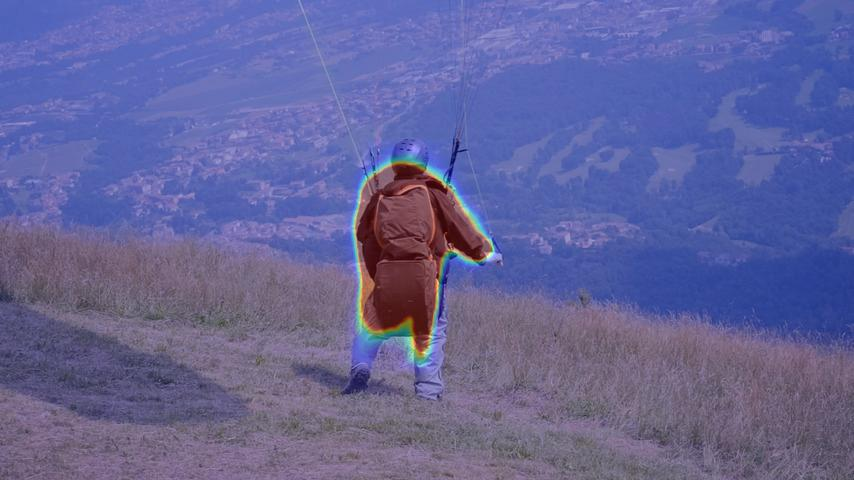
\includegraphics[width=2.43cm]{images/davis16val/paragliding-launch/00001.jpg}}          \hspace{-0.6em}        
    \subfloat{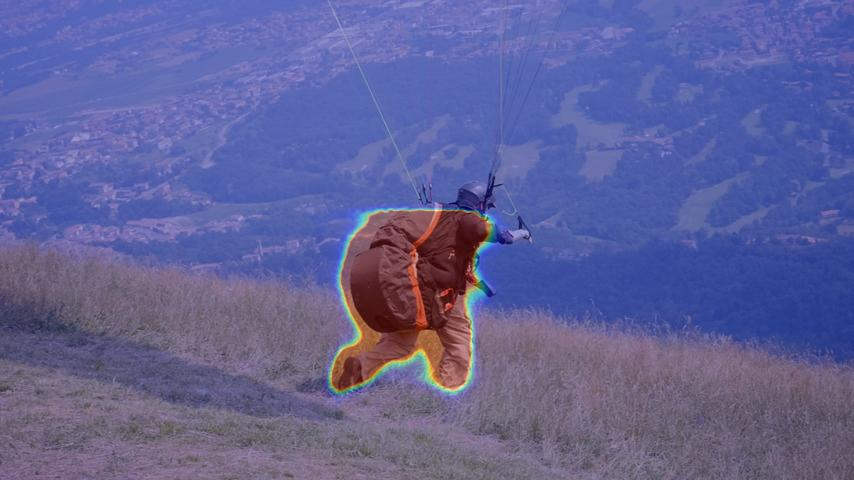
\includegraphics[width=2.43cm]{images/davis16val/paragliding-launch/00021.jpg}}          \hspace{-0.6em}        
    \subfloat{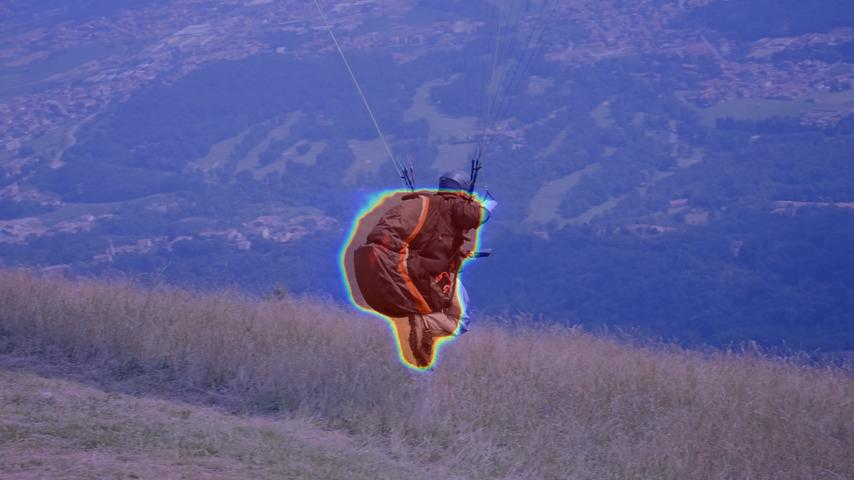
\includegraphics[width=2.43cm]{images/davis16val/paragliding-launch/00032.jpg}}          \hspace{-0.6em}        
    \subfloat{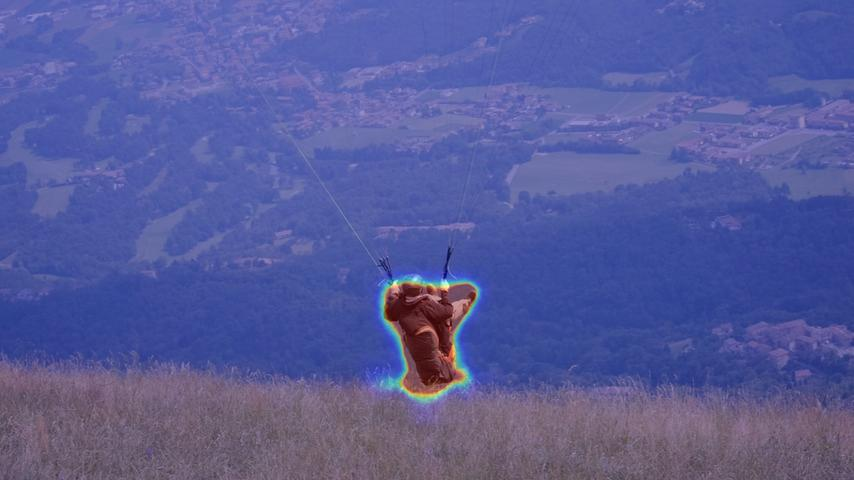
\includegraphics[width=2.43cm]{images/davis16val/paragliding-launch/00069.jpg}}          \hspace{-0.6em}        
    \subfloat{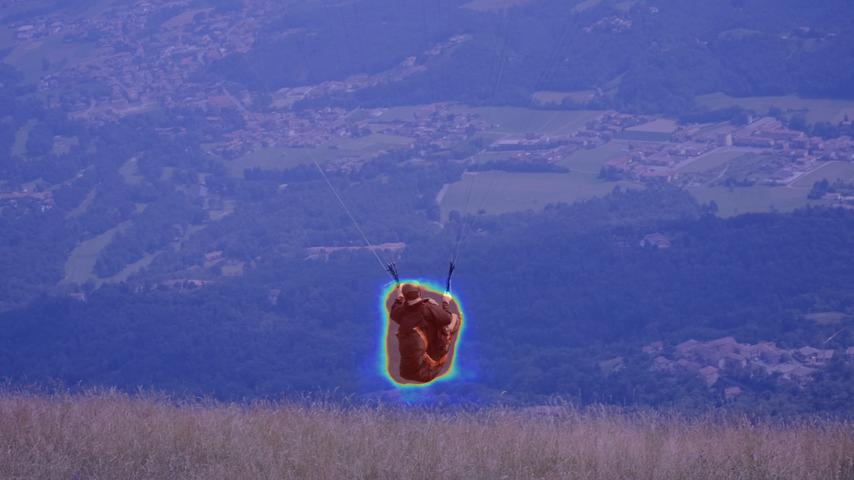
\includegraphics[width=2.43cm]{images/davis16val/paragliding-launch/00079.jpg}}\\[0.2ex]
    \subfloat{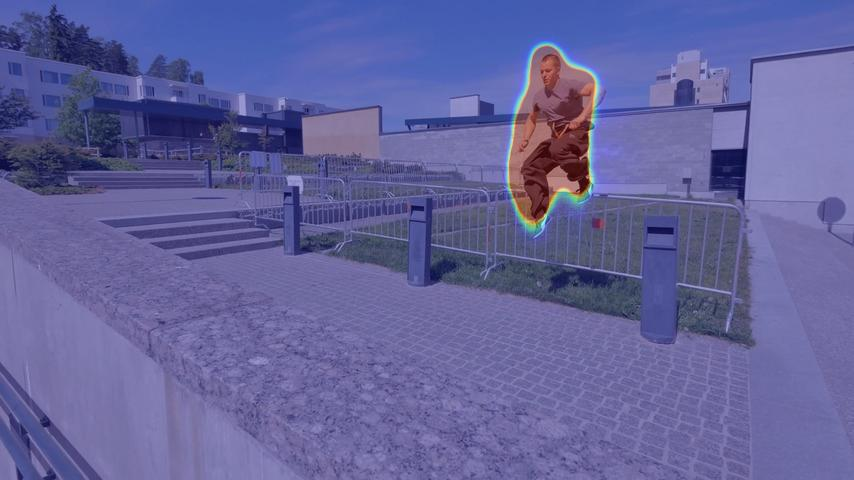
\includegraphics[width=2.43cm]{images/davis16val/parkour/00001.jpg}}                     \hspace{-0.6em}
    \subfloat{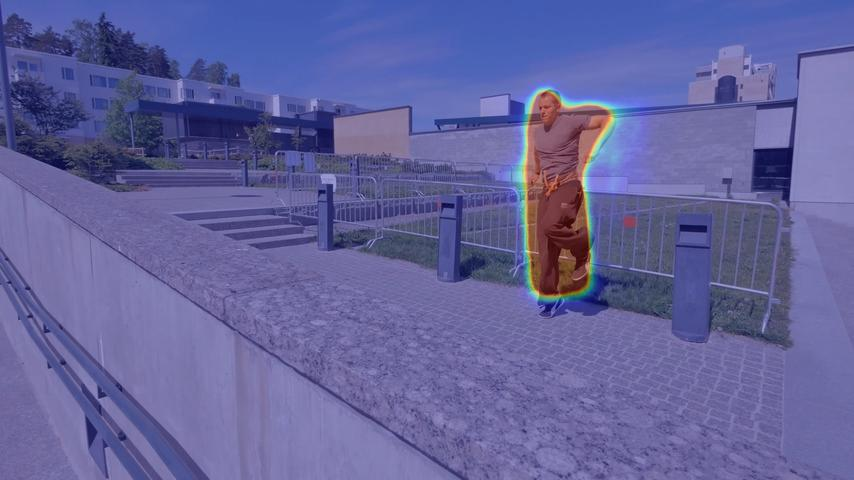
\includegraphics[width=2.43cm]{images/davis16val/parkour/00006.jpg}}                     \hspace{-0.6em}
    \subfloat{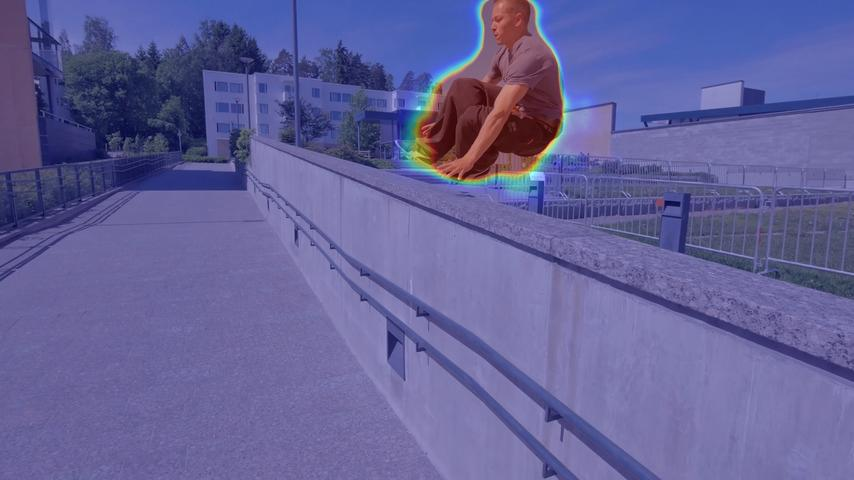
\includegraphics[width=2.43cm]{images/davis16val/parkour/00026.jpg}}                     \hspace{-0.6em}
    \subfloat{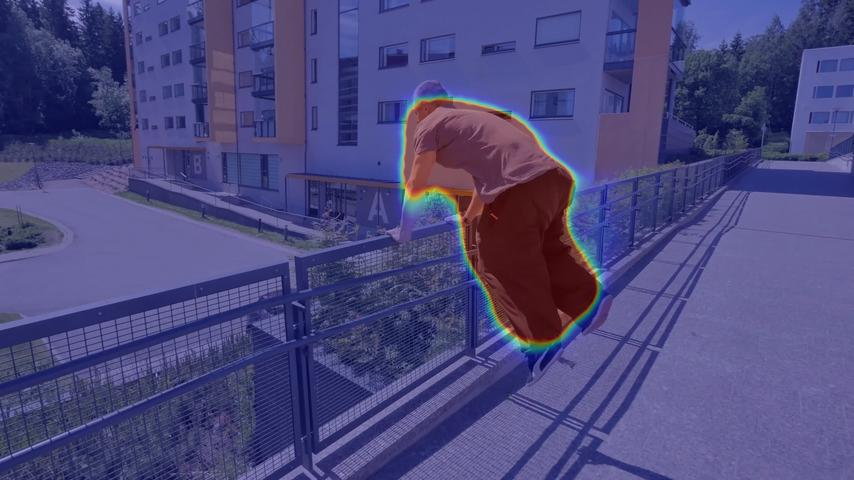
\includegraphics[width=2.43cm]{images/davis16val/parkour/00063.jpg}}                     \hspace{-0.6em}
    \subfloat{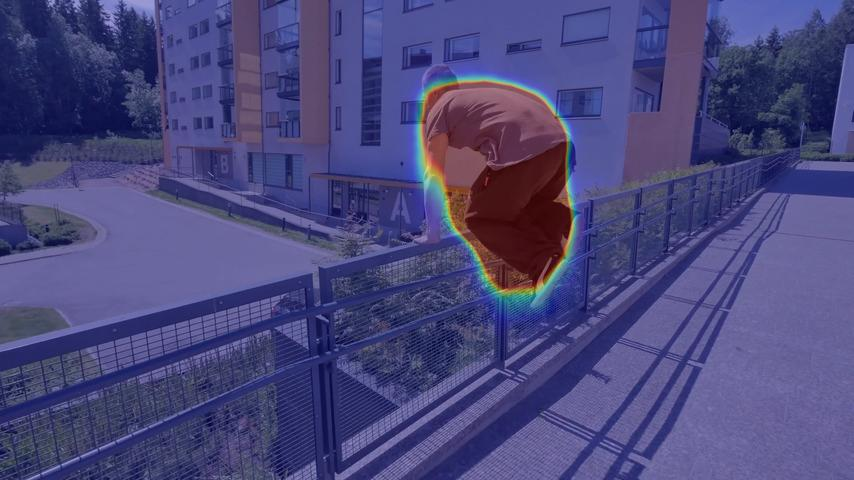
\includegraphics[width=2.43cm]{images/davis16val/parkour/00065.jpg}}\\[0.2ex]
    \subfloat{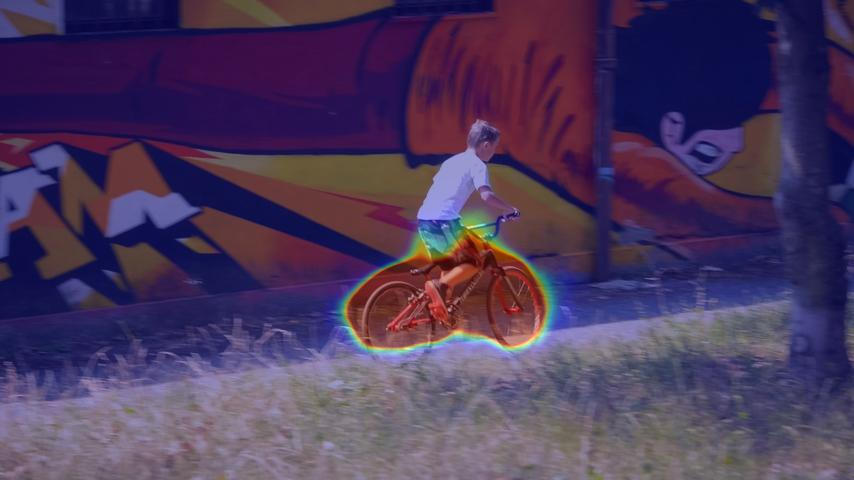
\includegraphics[width=2.43cm]{images/davis16val/bmx-trees/00001.jpg}}                   \hspace{-0.6em}
    \subfloat{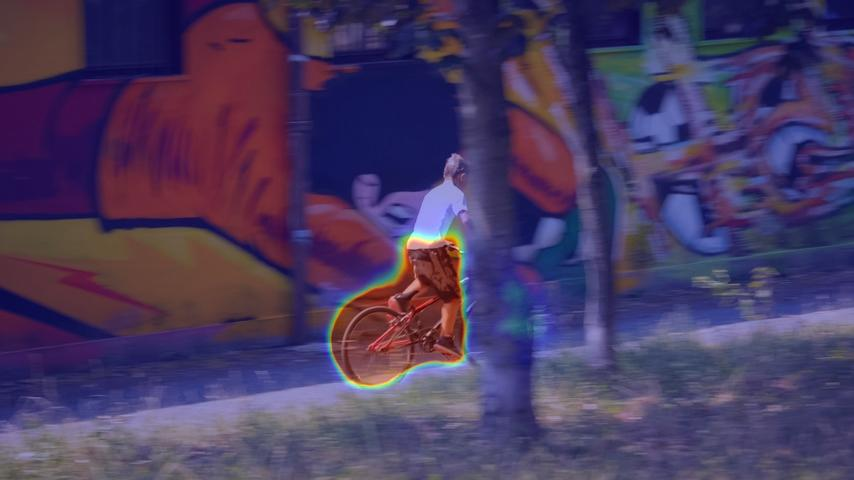
\includegraphics[width=2.43cm]{images/davis16val/bmx-trees/00014.jpg}}                   \hspace{-0.6em}
    \subfloat{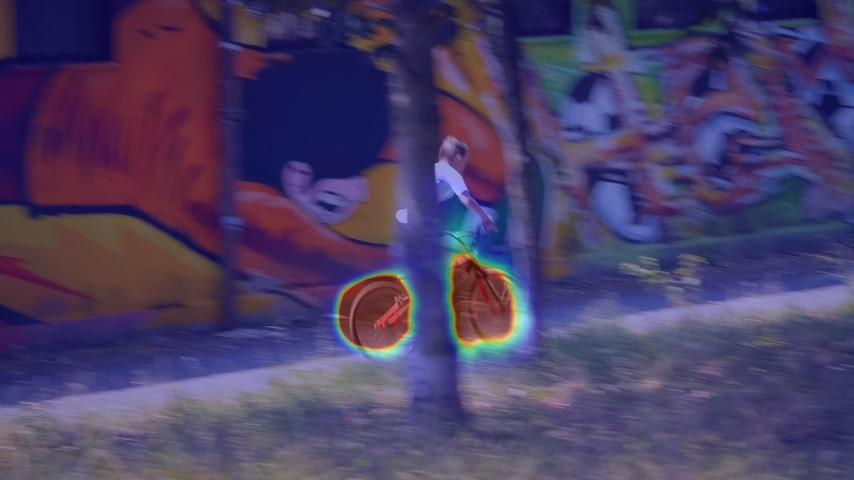
\includegraphics[width=2.43cm]{images/davis16val/bmx-trees/00017.jpg}}                   \hspace{-0.6em}
    \subfloat{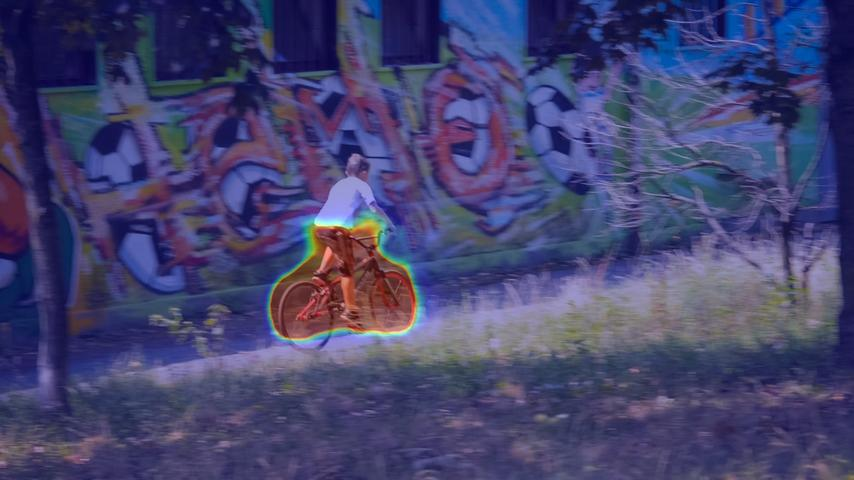
\includegraphics[width=2.43cm]{images/davis16val/bmx-trees/00036.jpg}}                   \hspace{-0.6em}
    \subfloat{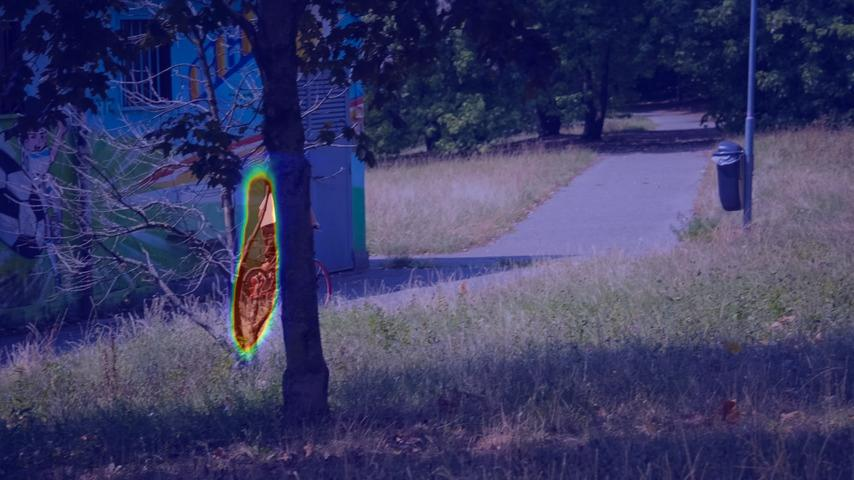
\includegraphics[width=2.43cm]{images/davis16val/bmx-trees/00067.jpg}}
    \caption{Qualitative results of our method in DAVIS2016 VAL dataset.}
    \label{fig:davis}
\end{figure}


\subsection{Evaluation on DAVIS2016}
Equipped with the InstMask module, the proposed tracker not only performs target tracking well, but it can also be used for video segmentation. DAVIS \cite{Perazzi2016} is a video object segmentation dataset, which consists of fifty high quality video sequences, spanning multiple occurrences of common video object segmentation challenges such as occlusions, motion blur and appearance changes. We performed qualitative experiments on the validation set of DAVIS2016. The visualization results are shown in Fig. \ref{fig:davis}. The results show that the proposed IGCF can accurately recover the contour of a target, which explains to some extent why IGCF can achieve performance improvement in tracking.

\section{Conclusion}
In this paper, we propose a novel target tracker which combines the advantages of deep neural networks and correlation filters to improve the performance of object tracking.
The InstMask is used to constrain the learning process of correlation filters. Based on the instance-level segmentation, we further propose a self-correction mechanism to mitigate the drift to the correlation filter.
Experiment results exhibit the superior robustness and efficiency of the proposed method by comparing it with state-of-the-art trackers.

\end{CJK*}

\section*{References}

\bibliography{mybibfile}

\end{document}